\documentclass[a0,portrait]{a0poster}

\usepackage{multicol} % This is so we can have multiple columns of text side-by-side
\columnsep=100pt % This is the amount of white space between the columns in the poster
\columnseprule=2pt % This is the thickness of the black line between the columns in the poster
\usepackage{times}
\usepackage[font=small,labelfont=bf]{caption}
\usepackage{wrapfig}
\usepackage{amsmath}
\usepackage{amsfonts}
\usepackage{amsthm}
\usepackage{bibentry}
\usepackage{graphicx}
\usepackage{bm}
\usepackage{booktabs}
\usepackage{tikz}
\usepackage{xcolor}
\usepackage{multirow}
\usepackage[normalem]{ulem}
\usepackage{pifont}
\usepackage{array}
\usepackage{sectsty}
% \allsectionsfont{\centering}
\graphicspath{{figures/}, {../images/}, {../auto_fig/}}

\definecolor{l10_color1}{HTML}{3232FF}
\definecolor{coloranswer}{HTML}{0596FF}
\definecolor{lightblue}{HTML}{3CC7EA}
\definecolor{boxcolor}{HTML}{EEEEEE}
\definecolor{periwinkle}{rgb}{0.8, 0.8, 1.0}
\definecolor{colorsquad}{rgb}{0,1,0}
\definecolor{colorsnli}{rgb}{1,0,0}
\definecolor{colorvqa}{rgb}{1,1,0}

\newcommand\BibTeX{B{\sc ib}\TeX}
\newcommand{\abr}[1]{\textsc{#1} }
\newcommand{\squad}{\textsc{SQuAD}}
\newcommand{\snli}{\textsc{SNLI}}
\newcommand{\vqa}{\textsc{VQA}}
\newcommand{\nlp}{\textsc{nlp}}
\newcommand{\mb}[1]{\boldsymbol{\mathbf{#1}}}
\newcommand{\loo}{leave-one-out}
\newcommand{\g}{\, | \,}

\begin{document}

%----------------------------------------------------------------------------------------
%	POSTER HEADER 
%----------------------------------------------------------------------------------------

% The header is divided into two boxes:
% The first is 75% wide and houses the title, subtitle, names, university/organization and contact information
% The second is 25% wide and houses a logo for your university/organization or a photo of you
% The widths of these boxes can be easily edited to accommodate your content as you see fit

\begin{minipage}[b]{1\linewidth}
\centering
\veryHuge \color{blue} \textbf{Pathologies of Neural Models Make Interpretation Difficult} \\[0.4cm]
\color{black}\LARGE
Shi Feng$^1$ Eric Wallace$^1$ Alvin Grissom~II$^2$ Mohit Iyyer$^{3,4}$ Pedro Rodriguez$^1$ Jordan Boyd-Graber$^1$\\[0.4cm]
\Large
\textit{$^1$University of Maryland $^2$Ursinus College $^3$UMass Amherst $^4$Allen Institute for Artificial Intelligence}\\
\end{minipage}

\vspace{0.3cm}

\begin{multicols}{2}

\large

\section*{Abstract}
\begin{itemize}
\item We interpret text classifiers by highlighting important words in the input.
\item The highlights are usually computed based on model confidence.
\item We use input reduction to expose pathologies of model confidence;
\item explain why this makes interpretation difficult;
\item and propose a simple mitigation.
\end{itemize}
\vspace{0.3cm}

\section*{Pathological Examples}
Neural model confidence is known to have issues. Here we show a particular case:
models making the same predictions with high confidence even when the inputs are
reduced to only a few words and appear non-sensical to humans.
\vspace{0.3cm}
\begin{center}
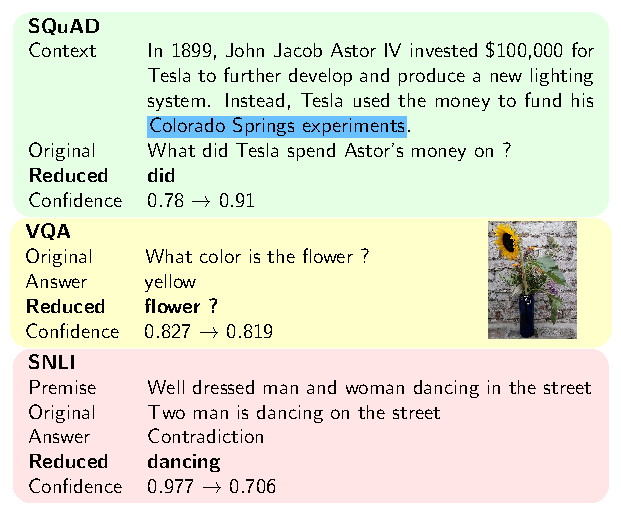
\includegraphics[width=\linewidth]{21}
\vspace{0.3cm}
\end{center}

\section*{Interpretation with Leave-One-Out}
\begin{itemize}
\item Saliency maps indicate the ``importance'' of each word to the model's prediction.
\item Simple importance function: remove each word and measure the confidence decrease.
\end{itemize}
\vspace{0.3cm}
\begin{center}
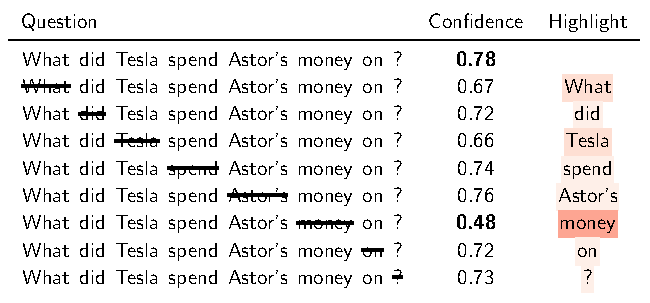
\includegraphics[width=\linewidth]{9}
\end{center}
\vspace{0.3cm}

\section*{Input Reduction}
\begin{itemize}
\item The way we generate the pathological examples follow the same principle.
\item We iteratively remove the least important words from the input.
\end{itemize}
\vspace{0.3cm}
\begin{center}
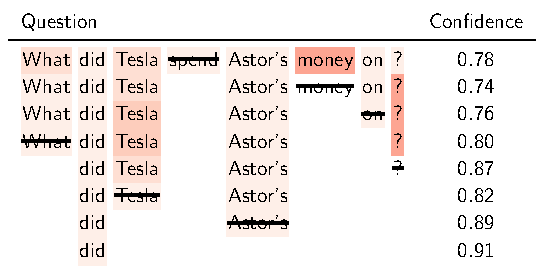
\includegraphics[width=\linewidth]{15}
\end{center}
%\vspace{0.3cm}

% \vfill\null
% \columnbreak

\section*{Reduced Examples Are Extremely Short}
\begin{itemize}
\item All examples in the validation set can be drastically reduced.
\item Model confidence remains high.
\end{itemize}
\begin{center}
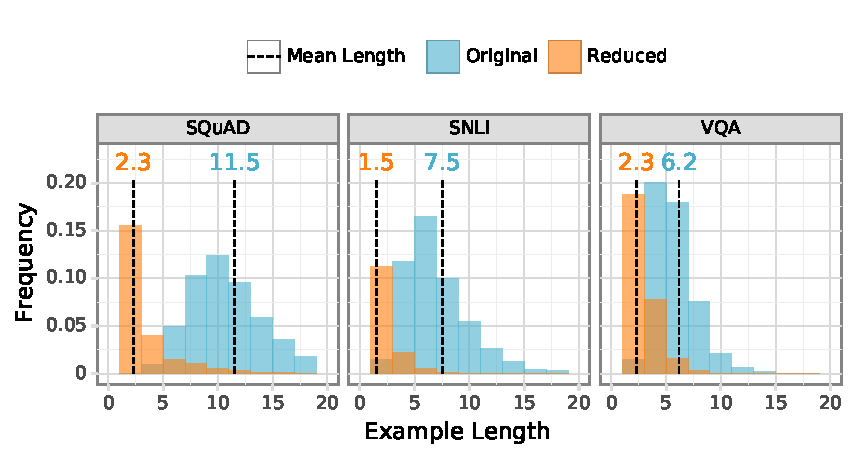
\includegraphics[width=0.9\linewidth]{length_histogram}
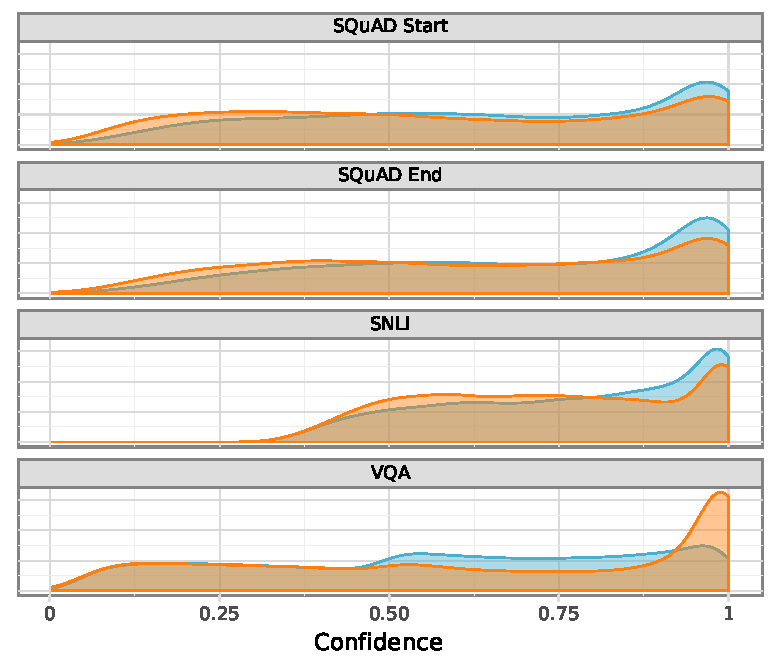
\includegraphics[width=0.7\linewidth]{confidence}
\end{center}

\section*{Reduced Examples Are Non-sensical}
\begin{itemize}
\item And the reduced examples are not just short but also non-sensical to humans.
\end{itemize}
\begin{center}
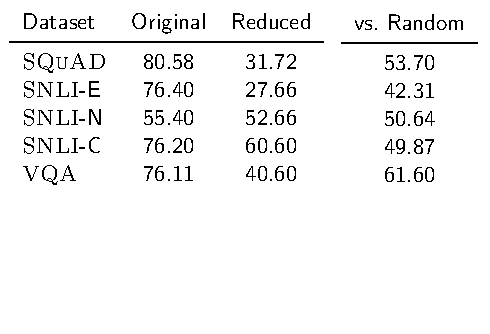
\includegraphics[width=0.8\linewidth]{29}
\end{center}

\section*{Heatmap Shifts}
\begin{itemize}
\item Importance is measured for each word individually.
\item High-order correlations between between words are ignored.
\item Removing an unimportant words can lead to a significant drop in the
    importance of an important word.
\end{itemize}
\begin{center}
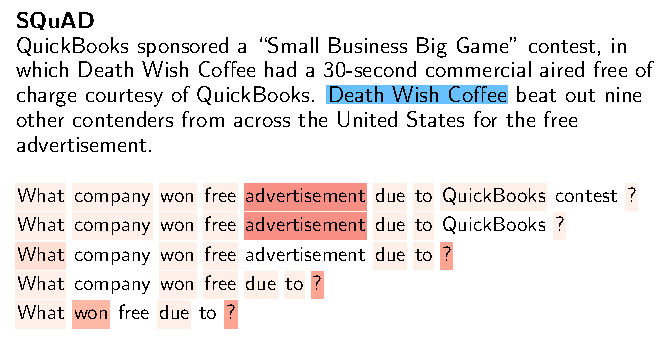
\includegraphics[width=0.9\linewidth]{42}
\end{center}

\section*{Mitigation}
\begin{center}
\begin{equation}
\sum_{(\mb{x}, y)}\log(f(y \g \mb{x})) \
+ \lambda\sum_{\tilde{\mb{x}}\in \tilde{\mathcal{X}}}
\mathbb{H}\left(f(y \g \tilde{\mb{x}})\right) \nonumber
\end{equation}
\end{center}
\begin{itemize}
\item Treat reduced examples as negative.
\item Models should not confidently predict any label.
\item Maximize the entropy on reduced examples.
\end{itemize}


% \vspace{0.6cm}
% 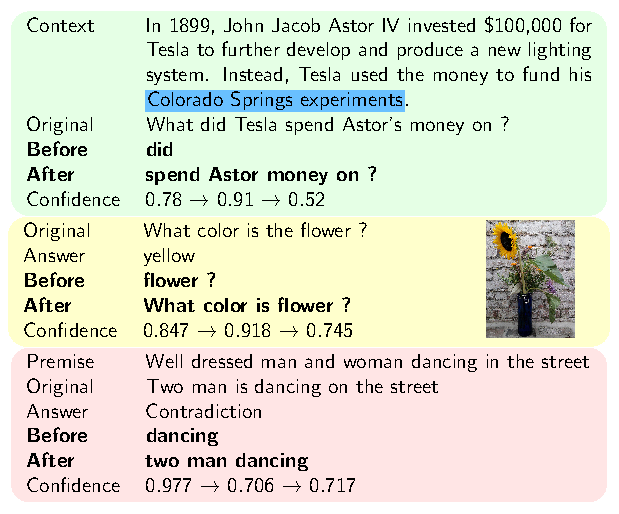
\includegraphics[width=0.9\linewidth]{48}
% \vspace{0.6cm}
% 
% \vspace{0.6cm}
% 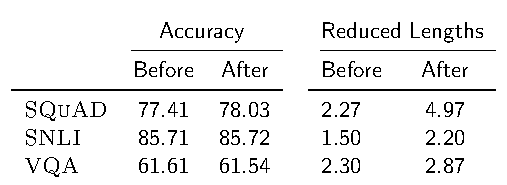
\includegraphics[width=0.9\linewidth]{50}
% \vspace{0.6cm}
% 
% \vspace{0.6cm}
% 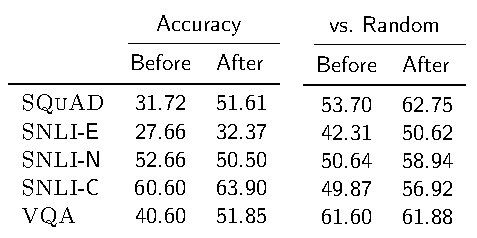
\includegraphics[width=0.9\linewidth]{57}
% \vspace{0.6cm}


% \section*{Conclusions}
% \begin{itemize}
% \item Confidence of a neural model trained with MLE is not reliable for
% interpretation
% \item Existing interpretation methods ignore high-order correlation between
% words
% \end{itemize}

% \section*{Referencias}
% \bibliographystyle{plain} % Plain referencing style
% \bibliography{journal-abbrv,fs}

\end{multicols}
\end{document}
